% !TEX encoding = UTF-8
% !TEX TS-program = pdflatex
% !TEX root = computabilità e algoritmi.tex
% !TEX spellcheck = it-IT

\subsection{Calcolo della durata e del lavoro}\label{calcolo-della-durata-e-del-lavoro}

Il calcolo del lavoro è semplice, basta andare a contare tutte le porzioni di codice sequenziale.

Per calcolare la durata è necessario tenere conto se due attività possono essere eseguite in parallelo

\begin{figure}[htbp]
\centering
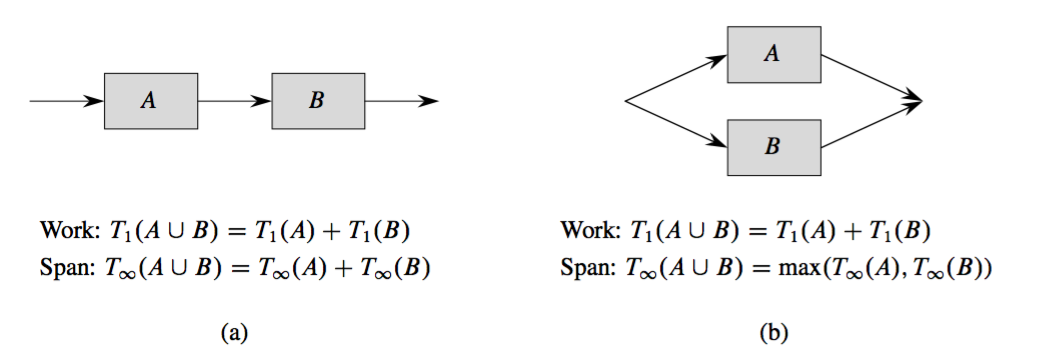
\includegraphics[width=.8\textwidth]{./notes/immagini/l25-fig1.png}
\caption{}
\end{figure}

Se due computazioni devono essere eseguite in sequenza la durata è la somma dei $T_\infty$ delle due compitazioni. Se invece possono essere eseguite in parallelo, la durata è il massimo dei due $T_\infty$.

\subsection{Loop paralleli}\label{loop-paralleli}

Moltiplicazione di un vettore per una matrice di dimensione $n \times n$

\begin{breakablealgorithm}
	\caption{\textsc{MatVec}: Moltiplicazione di una matrice per un vettore}
	\begin{algorithmic}[1]
\Function{MatVec}{$A,x$}
    \State $n \gets A.rows$
    \State $y\gets Vec(n)$
    \State \textbf{parallel}
    \For{$i = 1 \text{ to } n$}
        \State $y_i \gets 0$
    \EndFor
    \State \textbf{parallel}
    \For{$i = 1 \text{ to } n$}
         \For{$j = 1 \text{ to } n$}
            \State $y_i \gets y_i + a_{i,j}x_j$
        \EndFor
    \EndFor
\EndFunction
\end{algorithmic}
\end{breakablealgorithm}


Per quanto riguarda il lavoro si ha $T_1(n) = \Theta(n^2)$.

La durata invece $T_\infty(n)$ si ha che il primo blocco \textbf{parallel} ha durata $\Theta(\log n )$, perché il ciclo di azzeramento viene ottimizzato dalla piattaforma parallela in qualcosa di simile a:

\begin{breakablealgorithm}
\begin{algorithmic}[1]
\Function{Azzera}{$y,i,j$}
\If{$i = j$}
    \State $y_i \gets 0$
\Else 
    \State $m \gets \lfloor (i+j)/2\rfloor$
    \State \textbf{spawn} \textsc{Azzera}$(y,i,m)$
    \State \textsc{Azzera}$(y,m+1,j)$
    \State \textbf{sync}
\EndIf
\EndFunction
\end{algorithmic}
\end{breakablealgorithm}

Il lavoro di questa procedura in funzione di $n = j-i+1$ è $T_1(n)= 2T_1(n/2)+ C = \Theta(n)$. $T_\infty(n)$ è invece uguale a $T_\infty(n/2)+C = \Theta(\log(n))$ che deve essere sommata alla durata del blocco, che in questo caso è costante.

Si ha quindi che quando viene calcolata la durata di un \textbf{parallel for} c'è da tenere in considerazione un $\Theta(\log n )$ dovuto al lavoro svolto dalla piattaforma parallela per parallelizzare le istruzioni.

In modo simile a prima il secondo blocco ha complessità $\Theta(\log n ) +\Theta(n) = \Theta(n)$.

Si ha quindi che quando c'è un parallel c'è sempre una costante $\log n$ da sommare alla complessità a causa dell'implementazione del for.

$T_\infty$ di tutto l'algoritmo è quindi $\Theta(n)$.

\subsection{Race condition}\label{race-condition}

Se l'esecuzione dell'algoritmo fornisce sempre lo stesso risultato viene detto \textbf{deterministico} e questo avviene quando l'ordine di esecuzione degli strand non è influente sul risultato.

Se invece l'ordine è influente sul risultato si ha che l'algoritmo è \textbf{non deterministo} e questo può essere causato da delle \textbf{race condition} ovvero quando due strand eseguiti in parallelo accedono alla stessa locazione di memoria.

Ci sono vari modi per evitare queste situazioni, noi ci limitiamo ad analizzare del codice che non le prevede, ovvero che tutte le operazioni eseguite in parallelo sono tra loro \textbf{indipendenti}.

\subsection{Una lezione di scacchi}\label{una-lezione-di-scacchi}

Un algoritmo parallelo è stato progettato per lavorare con $p = 32$ e con
un $T_{32} = 65 $ secondi.

Si è poi riusciti a ridurre il tempo di esecuzione a $T'_{32} = 40$ secondi.

Tuttavia una volta eseguito il codice con $p = 512$ la seconda versione dell'algoritmo è risultata meno performante.

La versione originale aveva $T_1 = 2048$ e $T_\infty = 1$, mentre quella modificata aveva $T'_1 = 1024$ e $T_\infty = 8$. Ovvero la seconda versione ha dimezzato il lavoro, ma ha aumentato la durata.

Per il programma originale, utilizzando $T_P = T_1/P + T_\infty$:

$$T_{32} = 2048/32 +1 = 65 \quad \text{e} \quad T'_{32} = 1024/32 +8 = 40$$

mentre

$$T_{512} = 2048/512 + 1 = 5 \quad \text{e} \quad  T_{512} = 1024/512 + 8 = 10$$

Morale della favola, diminuire il lavoro non sempre porta ad una riduzione della durata.

\section{Moltiplicazione di due matrici}

\begin{breakablealgorithm}
	\caption{\textsc{P-Square-Matrix-Multiply}: moltiplicazione di due matrici parallelizzata}
	\begin{algorithmic}[1]
		\Function{P-Square-Matrix-Multiply}{A,B}
			\State $n \gets A.rows$
			\State $C \gets n \times n $ Matrix
			\State \textbf{parallel}
			\For{$i = 1 \textbf{ to } n$}
				\State \textbf{parallel}
				\For{$j = 1 \textbf{ to } n$}
					\State $C_{i,j} \gets 0$
					\For{$k = 1 \textbf{ to } n$}
						\State $C_{i,j} \gets C_{i,j} + a_{i,j} \cdot B_{i,j}$
					\EndFor
				\EndFor
			\EndFor
			\State \Return $C$
		\EndFunction
	\end{algorithmic}
\end{breakablealgorithm}

Il lavoro svolto da questo algoritmo è lo stesso delle versione sequenziale, si ha quindi $T_1(n) = \Theta(n^3)$.

Per quanto riguarda la durata, c'è un tempo costante per l'inizializzazione delle matrice, due complessità logaritmiche per i due loop paralleli innestati e un $\Theta(n)$ per il for non parallelo. Si ha quindi:

\begin{align*}
	T_\infty(n) &= O(1) + \Theta(\log n) + \Theta(\log n) + \Theta(n) \\
		&= \Theta(n)
\end{align*}

Il parallelismo è quindi $\Theta(n^2)$ e può essere migliorato utilizzando l'approccio divide-and-conquer del metodo di Strassen.

Da notare che il terzo ciclo for di questo algoritmo non può essere parallelizzato perché altrimenti si creerebbero delle race condition.

\section{Merge Sort}\label{merge-sort}

La versione sequenziale dell'algoritmo prende un array \emph{A} e due indici \emph{p} e \emph{r} e deve ordinare la porzione dell'array compresa tra \emph{p} e \emph{r}.

\begin{breakablealgorithm}
	\begin{algorithmic}[1]
\Function{MergeSort'}{$A,p,r$}
\If{$p < r$}
    \State $q \gets floor(p+r/2)$
    \State \textbf{spawn } \textsc{MergeSort'}$(A,p,q)$
    \State \textsc{MergeSort'}$(A,q+1,r)$
    \State \textbf{sync}
    \State \textsc{Merge}$(A,p,q,r)$
\EndIf
\EndFunction
	\end{algorithmic}
\end{breakablealgorithm}

Il lavoro $T_1(n)$ è $\Theta(n \log n)$ che deriva dalla versione sequenziale del \textsc{MergeSort}.

La durata è invece uguale ad un tempo costante, più la massima durata delle chiamate ricorsive, che possono essere considerate uguali, più la durata del merge, che se viene fatto in modo sequenziale è $\Theta(n)$. 

Si ha quindi che 

$$T_\infty = T_\infty(n/2) + \Theta(n) = \Theta(n)$$ 

(\emph{per il metodo dell'esperto o qualcosa del genere}).

Il parallelismo di questo algoritmo risulta quindi essere $\Theta(\log n)$ che non è buono.

Questo perché nell'ordinamento di un numero elevato di elementi, si riesce a raggiungere uno speedup lineare con pochi processori, ma all'aumentare del numero dei processori l'algoritmo non scala.

Per aumentare il parallelismo è necessario rendere parallela anche la funzione \textsc{Merge}.

\begin{figure}[htbp]
\centering
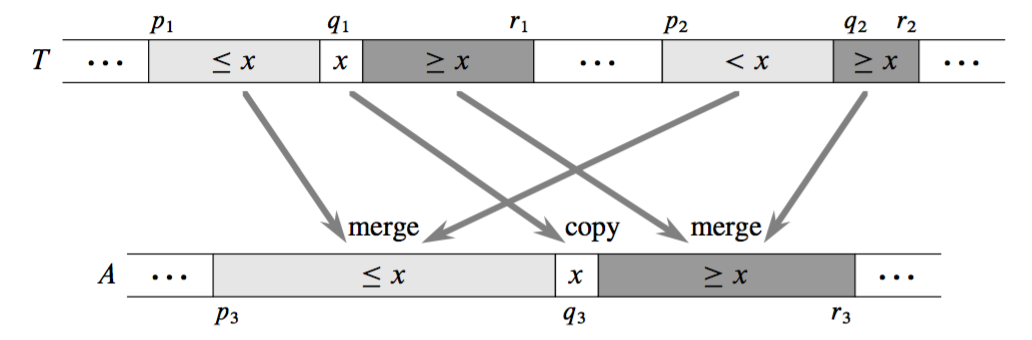
\includegraphics[width=.8\textwidth]{./notes/immagini/l25-fig2.png}
\caption{\textsc{Merge} parallelo}
\end{figure}

Supponiamo che nell'array \emph{T} risultante dalle due chiamate ricorsive ci siano due porzioni ordinate che vanno rispettivamente da $p_1$ a $r_1$ e da $p_2$ a $r_2$.

L'idea è quella di prendere la parte più lunga dei due segmenti. 
Se questa è lunga 0, sono entrambi vuoti e non è necessario fare niente.

Se invece è più lunga di 0, viene calcolato l'indice $q_1$ dell'elemento mediano della prima parte,
ovvero l'elemento centrale della sequenza, il quale avrà un certo valore \emph{x}.

La seconda sequenza può quindi essere divisa in altre due sotto-sequenze, una contenente solo valori minori di \emph{x} e un'altra con tutti i valori $\geq x$. 
Il primo elemento $\geq x$ avrà un certo indice $q_2$ e può essere trovato utilizzando una ricerca binaria in tempo logaritmico.

Da notare che $q_2$ può essere uguale a $p_2$ se sono tutti maggiori uguali di $x$ o a $r_2+1$ se sono tutti minori.

Si sa quindi che, una volta ordinato il vettore, l'elemento \emph{x} si troverà nella posizione $q_3 = p_3 + (q_1-p_1) + (q_2-p_2)$ e può essere già scritto.

Si possono poi unire ricorsivamente tutti gli elementi minori di \emph{x}, ovvero quelli che vanno da $p_1$ a $q_1-1$ e da $p_2$ a $q_2-1$ , e tutti quelli maggiori uguali di $x$, ovvero quelli che vanno da $q_1$ a $r_1$ e da $q_2$ a $r_2$.

Dal momento che i primi andranno a finire nelle posizioni da $q_3$ a $q_3-1$ e i secondi andranno a finire nelle posizioni da $q_3+1$ a $r_3$, le due chiamate ricorsive possono essere parallelizzate.
